The measurement of cosmic distances is central to our understanding of
cosmography, i.e. the description of the geometry and kinematics of
the universe. The discovery of the period luminosity relation for
Cepheids led to the realization that the universe is much bigger than
the Milky Way and that it is currently expanding. Relative distance
measurements based on supernova Ia light curves were the turning point
in the discovery of the acceleration of the universe
\citep{Riess:1998p21184,Per++99}.

In the two decades since the discovery of the acceleration of the
universe, distance measurements have improved steadily. For example,
the Hubble constant has now been measured to 2.4\% precision
\citep{Rie++16} while the distance to the last scattering surface of
the cosmic microwave backgrond is now known to approximately 0.5\%
precision \citep[depending on the assumed cosmological
model]{WMAP9,Pla15}. This precision is more than sufficient for all
purposes related to our understanding of phenomena occurring within
the universe, like galaxy evolution.

In spite of all this progress, the most fundamental question still
remains unanswered. What is causing the acceleration? Is this {\it
dark energy} something akin to Einstein's cosmological constant or is
it a dynamical component? Answering this question from an empirical
standpoint will require further improvements in the precision of
distance measurements \citep{Suy++12,Wei++13,Kim++15,Rie++16}.  In
practice, measuring the dark energy equation of state requires an
accurate model of the scale parameter of the universe as a function of
time, particularly when dark energy is dynamically most relevant,
i.e. below $z\sim1$.

%\begin{figure}[!t]
%\begin{center}
%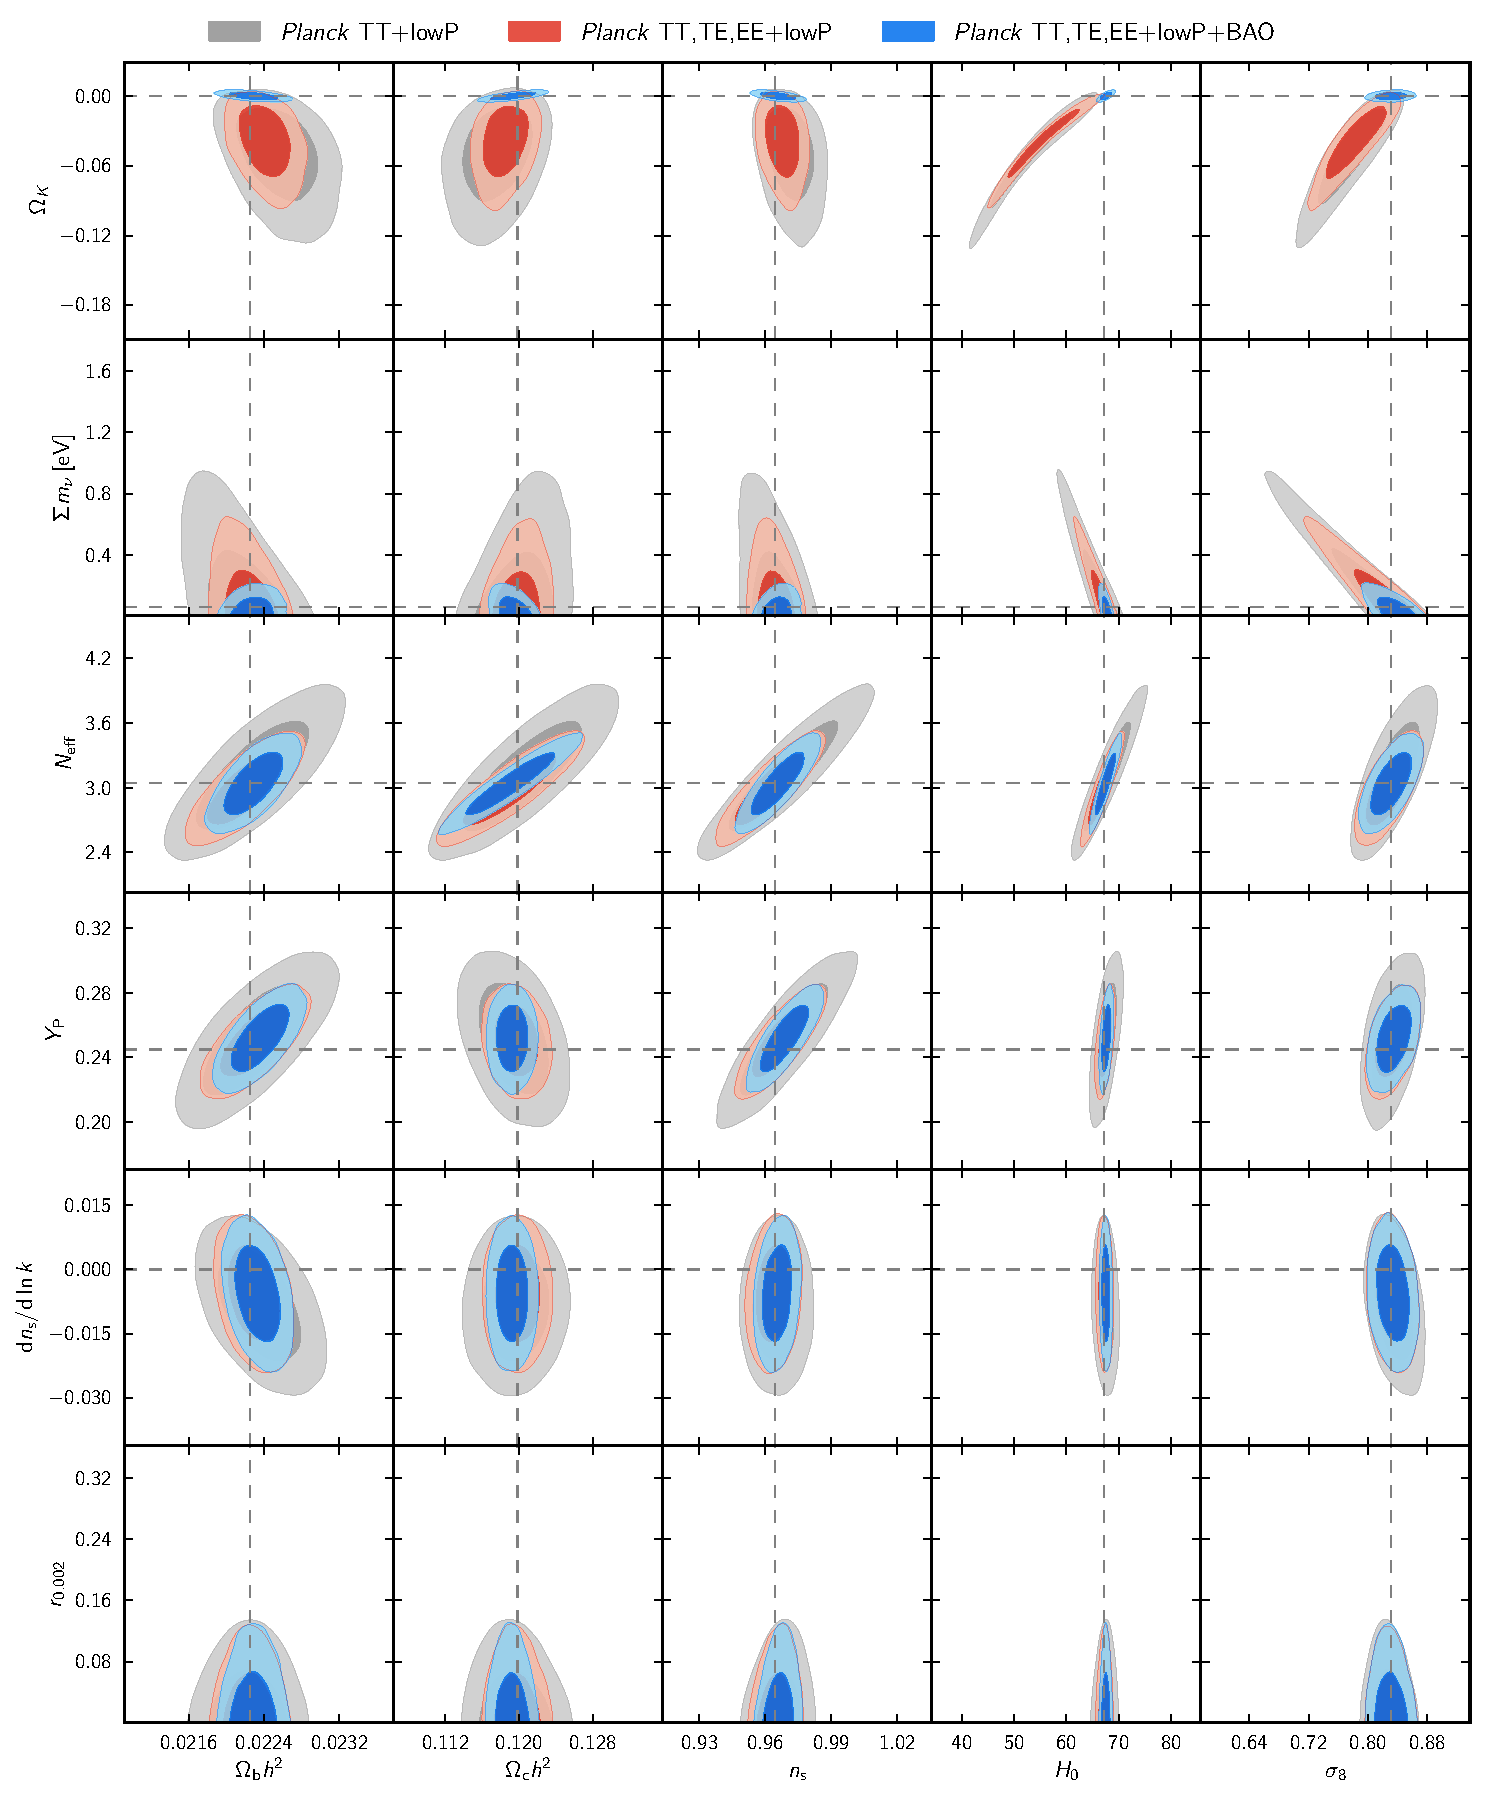
\includegraphics[width=0.5\textwidth]{figures/grid_1paramext.pdf}
%\caption{The figure, taken from \cite{Pla15}, shows the confidence
%intervals obtained for 1-parameter extension of the basic $\Lambda$CDM
%model obtained using Plank measurements themselves, and in combination
%with baryonic acoustic oscillations. Note that the interpretation of
%CMB data long is strongly degenerate, even in these simple
%models. Lower redshift distance measurements, in case from BAO, break
%the degeneracies. See the original paper \cite{Pla15} for details
%about the figure and input parameters.}
%\label{fig:CMB}
%\end{center}
%\end{figure}

Cosmic microwave background anisotropies primarily provide a
measurement of the angular distance to the last scattering surface,
obtain by comparing the angular scale of the acoustic peaks with the
baryonic acoustic oscillation scale. Therefore, the constraints set by
CMB anisotropy data on dark energy parametere are highly degenerate in
a generic cosmological model
\citep[e.g.,][]{Pla15}. Breaking the degeneracy requires strong
assumptions about the universe (e.g., flatness or dark energy being
the cosmological constant), or lower redshift distance
measurements. Many dedicated experiments are currently under way or
being planned with this goal in mind.

%A summary of distance
%measurements with approximate precision and redshift range is given in
%Figure~\ref{fig:comparedist}.
%[Include distance ladder, CMB, BAO, cosmic clocks, fgas]

%\begin{figure}[!t]
%\begin{center}
%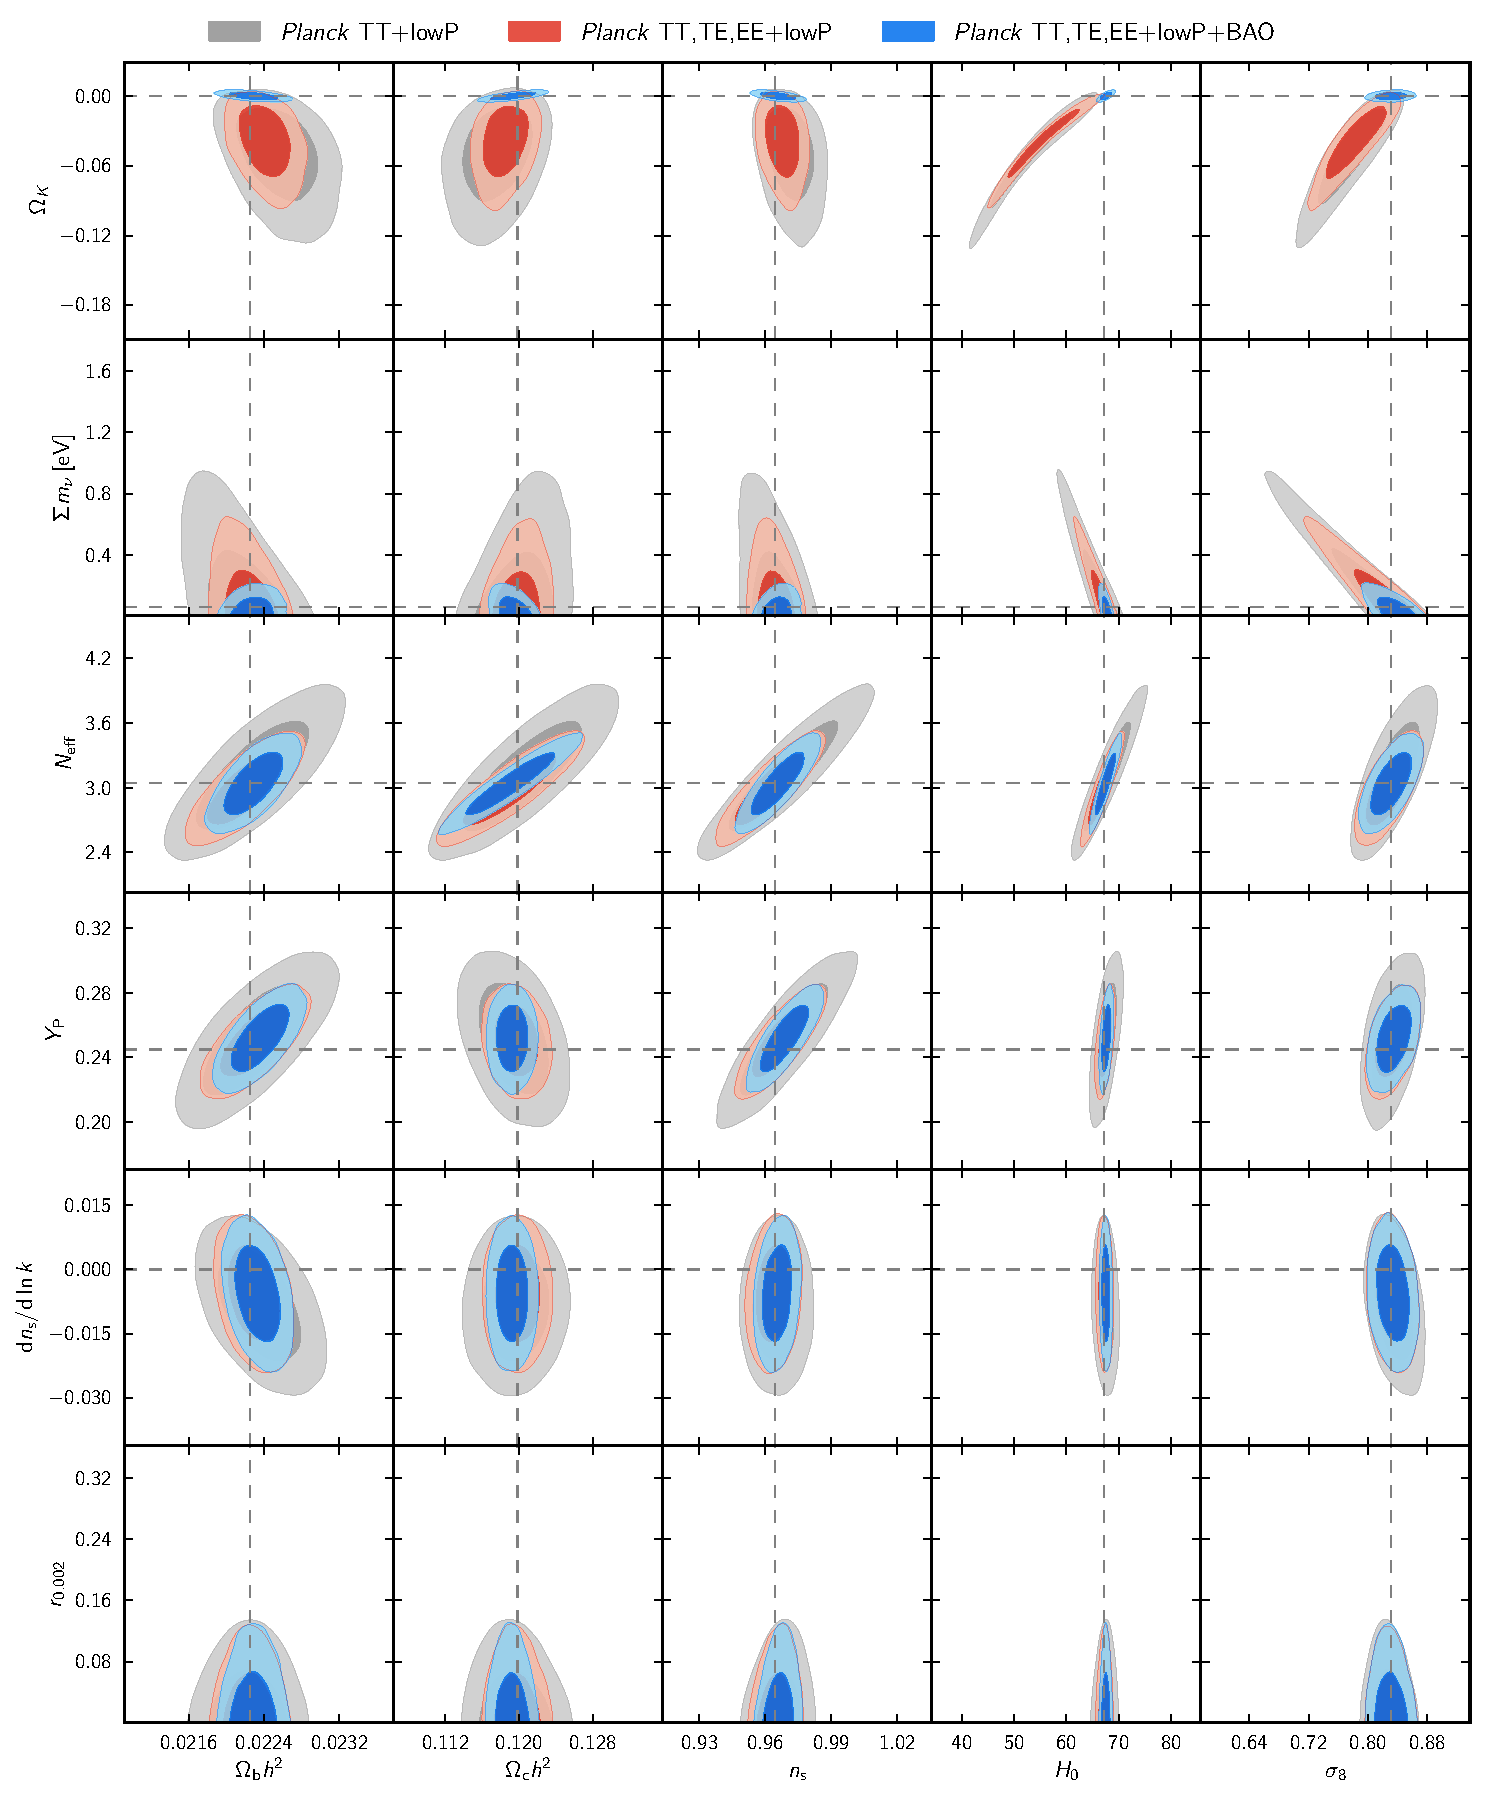
\includegraphics[width=0.5\textwidth]{figures/grid_1paramext.pdf}
%\caption{Summary of current distance measurements}
%\label{fig:comparedist}
%\end{center}
%\end{figure}

Precision, however, is not sufficient by itself. In addition to
controlling the known statistical uncertainties ({\it precision}),
modern day experiments need to control systematic errors ({\it
accuracy}) in order to fullfill their potential, including the
infamous unknown unknowns. The most direct way to demonstrate accuracy
is to compare independent measurements that have comparable precision. An
interesting, currently topical, and relevant case is that of the 3$-\sigma$ tension
between the local distance ladder determination of H$_0$
\citep{Rie++16} and that inferred by the Plank satellite assuming a
flat $\Lambda$CDM model \citep{Pla15}. The tension could be due to an
unknown source of systematic errors in either or both of the two measurements, or
it could be indicative of new physics, for example an effective number of
relativistic species greater than three. Independent measurements with
comparable precision are the best way to make progress.
% For example,
% the WMAP9 measurement \citep{Cal++13} is significantly less in tension
% with the cosmic distance ladder data than the Planck one.
While independent measurements of the same phenomenon, or reanalysis of the
same data \citep{Efs14,SFH15}, are certainly useful and necessary,
completely independent datasets based on different physical phenomena
provide qualitatively new information.

Ideally, the comparison between independent measurements should be
carried out blindly, so as to minimize experimenter bias. Two mutually
blind measurements agreeing that the equation of state parameter $w$
is not $-1$ would be a very convincing demonstration that the dark
energy is not the cosmological constant. Conversely, the significant
disagreement of two blind and independent measurements, could be the
first sign of new physics.

In this review we focus on strong lensing gravitational time delays as
a tool for cosmography. As we shall see, this probe provides a direct
and elegant way to measure absolute distances out to cosmological
redshift. When the line of sight to a distant source of light is
suitably well aligned with an intervening massive system, multiple
images appear to the observer. The arrival time of the images depends
on the interplay of the geometric and gravitational delays specific to
the configuration. If the emission from the source is variable in
time, the difference in arrival time is measurable, and can be
interpreted via a so-called ``time delay distance'' $\Ddt$.
In the simplest case, this distance is just a multiplicative combination
of the three angular diameter distances between the observer, deflector and
source. $\Ddt$ is
inversely proportional to the Hubble Constant $H_0$, and more
weakly dependent on other cosmological parameters. As several authors
have pointed out \citep{Hu05,Lin11,Suy++12,Wei++13}, achieving
sub-percent precision and accuracy on the measurement of the Hubble
constant will be a powerful addition to Stage III and IV dark energy
experiments. The independence of time delays from other traditional
probes of cosmology, makes them very valuable for precise and accurate
cosmology. For example, time delays yield an {\it absolute}
measurement of distance without relying on Cepheids or any other local
rung of the distance ladder, and because the relevant quantities are
angular diameter distances rather then luminosity distances, the
approach is insensitive to dust or
other photometric errors.

This review is organized as follows. In Section~\ref{sec:intro} we
summarize the history of time delay cosmography up until the turn of
the millennium, in order to give a sense of the early challenges and
how they were overcome. In Section~\ref{sec:theory}, we review the
theoretical foundations of the method, in terms of the gravitational
optics version of Fermat's principle. In Section~\ref{sec:measurement}
we describe in some detail the elements of a modern time delay
distance measurement, emphasizing recent advances and remaining
challenges. In Section~\ref{sec:cosmo} we elucidate the connection
between time delay distance measurements and cosmological parameters,
discussing complementarity with other cosmological
probes. Section~\ref{sec:outlook} critically examines the future of
the method, discussing prospects for increasing the precision, testing
for accuracy, and synergy with other future probes of dark energy. A
brief summary is given in Section~\ref{sec:summary}.

Owing to space limitations, we could only present a selection of all
the beautiful work that has been published on this topic in the past
decades. We refer the readers to recent
\citep{Bar10,Ell10,Tre10,TMC12,Jackson:2013p30763,Jac15,T+E15}
and not-so-recent \citep{B+N92,CSS02,K+S04,Fal05,SKW06}
excellent reviews and textbooks \citep{SEF92} for additional
information and historical context.
